% ====================================================================

% ====================================================================
\documentclass[article,paper=a4paper]{jlreq}

% jpreportパッケージの読み込み
\usepackage{jpreport}

% ページレイアウトの設定
\usepackage{geometry}
\usepackage{enumitem}
\geometry{
    top=20mm,
    bottom=20mm,
    left=20mm,
    right=20mm
}
% TikZライブラリ
\usetikzlibrary{
    patterns,
    calc,
    arrows,
    decorations,
    angles,
    shapes.geometric,
    fit,
    knots
}
% TikZ用のスタイル
\tikzset{
  every path/.style={
    black,
    line width=2pt
  },
  every node/.style={
    transform shape,
    knot crossing,
    inner sep=1.5pt
  }
}
% ハイパーリンクの設定
\usepackage[unicode]{hyperref}
\usepackage{bookmark}
\usepackage[nameinlink]{cleveref}

\hypersetup{
    colorlinks=true,
    linkcolor=black,
    urlcolor=blue,
    citecolor=blue,
    pdftitle=,
    pdfauthor=
}

% 数学演算子の定義


% cleveref用の日本語設定
\crefname{thm}{定理}{定理}
\crefname{lem}{補題}{補題}
\crefname{cor}{系}{系}
\crefname{ex}{例}{例}
\crefname{dfn}{定義}{定義}
\crefname{prop}{命題}{命題}
\crefname{prob}{問題}{問題}

% 色彩の定義
\definecolor{yukari}{RGB}{196, 163, 191}

% 文書情報
\title{幾何学1}
\author{akari0koutya}
\date{\today}

\begin{document}

% --- タイトル ------------------------------------------------------
\maketitle
\tableofcontents
%% 本文の内容をここに記述
% ====================================================================

\lecture{第1回 : (2026/04/14)}

\section{ガイダンス}

\subsection{注意点}

\begin{itemize}
    \item 第8回に中間試験、第15回に期末試験
    \item 成績評価は、中間試験 $35\%$、期末試験 $35\%$、レポート $30\%$
    \item 再試験なし
    \item 前半に距離空間を扱い、後半に位相空間を扱う
\end{itemize}

\subsection{アブストラクト}

ある集合を幾何学的な対象として扱うには、どういった情報があるとうれしいか。\par
$\longrightarrow$ 位相空間

距離が与えられている集合（\textbf{距離空間}）は、性質として強すぎる。たとえば、以下のような結び目も幾何学的対象として扱いたい:
\begin{figure}[htbp]
\begin{minipage}{0.45 \textwidth}
\centering
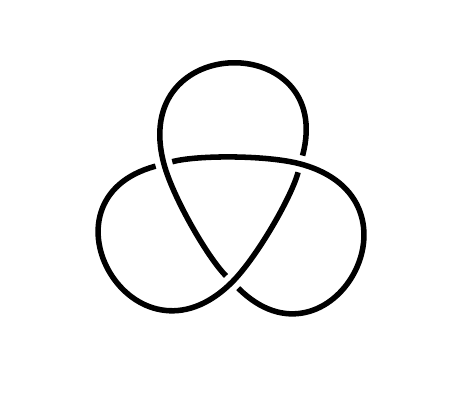
\begin{tikzpicture}
\foreach \brk in {0,1,2} {
\begin{scope}[rotate=\brk * 120]
\node (k\brk) at (0,-1) {};
\end{scope}
}
\draw (0,0) \foreach \brk in {0,1,2} {
    let \n0=\brk,
        \n1={int(Mod(\brk+1,3))},
        \n2={int(Mod(\brk+2,3))}
       in (k\n0) .. controls (k\n0.16 south east) and (k\n1.16 south west) .. 
          (k\n1.center) .. controls (k\n1.4 north east) and (k\n2.4 north west) .. 
          (k\n2)} (k2);
\end{tikzpicture}    
\end{minipage}
\begin{minipage}{0.45 \textwidth}
\centering

\begin{tikzpicture}
\foreach \brk in {0,...,4} {
\begin{scope}[rotate=\brk * 72]
\node (k\brk) at (0,-1) {};
\end{scope}
}
\draw (0,0) \foreach \brk in {0,...,4} {
    let \n0=\brk,
        \n1={int(Mod(\brk+1,5))},
        \n2={int(Mod(\brk+2,5))}
    in (k\n0) .. controls (k\n0.16 south east) and (k\n1.16 south west) .. 
       (k\n1.center) .. controls (k\n1.4 north east) and (k\n2.4 north west) .. 
       (k\n2)} (k2);
\end{tikzpicture}  
\end{minipage}   
\caption{結び目の例}  
\end{figure}

さて、2点 $x = (x_1, x_2, \ldots, x_n), y = (y_1, y_2, \ldots, y_n) \in \R^2$ に対し、
\begin{equation}
    d(x,y) = \sqrt{(x_1 - y_1)^2 + (x_2 - y_2)^2 + \cdots + (x_n - y_n)^2}
\end{equation}
とすれば、これは距離を定義することになる（\textbf{ユークリッド距離}）。これは、 $x$ と $y$ の線分の長さを表す。その他、京都の街やマンハッタンに見られる碁盤の目のような道にも距離も定義できる（\textbf{マンハッタン距離}）。このように、距離にも種類があり、多様な距離の定め方に通用する概念として距離を抽象化して考える。

\vspace{\baselineskip}

集合 $X$ に対し、距離が満たすべき性質として、以下の条件を考えられる:
\begin{itemize}
    \item $d(x,y) \geq 0$ かつ $d(x,y) = 0$ ならば $x=y$
    \item $d(x,y) = d(y,x)$
    \item $d(x,z) \leq d(x,y) + d(y,z)$ \quad （三角不等式）
\end{itemize}

\subsection{教科書}

\begin{itemize}
    \item 小山晃著, 位相空間論 : 現代数学への基礎, 森北出版, 2021.
\end{itemize}

\lecture{第2回 : (2026/04/21)}

\section{距離関数と距離空間}

\begin{dfn}
$X$ を集合、$d\colon X \times X \to \R$ を写像とし、以下の条件を満たすとする :
\begin{itemize}
    \item $d(x,y) = 0 \Leftrightarrow x=y$
    \item $d(x,y) = d(y,x)$
    \item $d(x,z) \leq d(x,y) + d(y,z)$ \quad （三角不等式）
\end{itemize}
このとき、$d$ を $X$ 上の\textbf{距離}と呼び、$(X,d)$ を\textbf{距離空間}と呼ぶ。
\end{dfn}

\begin{rem}
距離空間 $(X,d)$ の定義から直ちに導ける性質として次のものがある : 
\begin{itemize}
    \item 任意の $x,y \in X$ に対して、$d(x,y) \geq 0$ を満たす。
\end{itemize}
\end{rem}

\begin{rem}
距離空間 $(X,d)$ という表記を $X$ と省略して表記することもある。
\end{rem}

\begin{ex}
距離空間の例として、以下のものがある :
\begin{itemize}
    \item \textbf{ユークリッド距離} : $\R^n$ 上の距離を 
    \[d(x,y) = \sqrt{(x_1 - y_1)^2 + (x_2 - y_2)^2 + \cdots + (x_n - y_n)^2}\]
    と定めると、これは距離空間となる。\\
    \quad 実際、
    \begin{align*}
        d(x,y) = 0 &\Leftrightarrow (x_1 - y_1)^2 + (x_2 - y_2)^2 + \cdots + (x_n - y_n)^2 = 0 \\
        &\Leftrightarrow x_1 = y_1, x_2 = y_2, \ldots, x_n = y_n \\
        &\Leftrightarrow x = y
    \end{align*}
    であり、コーシー・シュワルツの不等式より、
    \begin{align*}
        d(x,z)^2 &= (x_1 - z_1)^2 + (x_2 - z_2)^2 + \cdots + (x_n - z_n)^2 \\
        &= ((x_1 - y_1) + (y_1 - z_1))^2 + \cdots + ((x_n - y_n) + (y_n - z_n))^2 \\
        &\leq 2((x_1 - y_1)^2 + \cdots + (x_n - y_n)^2) + 2((y_1 - z_1)^2 + \cdots + (y_n - z_n)^2) \\
        &= 2d(x,y)^2 + 2d(y,z)^2 \\
        &\leq 4(d(x,y) + d(y,z))^2
    \end{align*}
    \item $I = [0,1]$、
    \[C(I) := \{f \mid f\colon I \to \R \text{ は連続関数}\}\]
    とする。$C(I)$ 上の距離を、
    \[d(f,g) = \sup_{x \in I} \left\lvert f(x) - g(x)\right\rvert\]
    と定めると、これは距離空間となる。\\
    \quad ここで、$f,g \in C(I)$ に対し、$\left\lvert f(x) - g(x) \right\rvert$ は $I$ における連続関数のため、最大値・最小値の定理より、必ず最大値を取る点 $x_0 \in I$ が存在する。したがって、
    \[\sup_{x \in I} \left\lvert f(x) - g(x) \right\rvert = \left\lvert f(x_0) - g(x_0) \right\rvert\]
    となるので、$d(f,g)$ は距離空間の定義を満たす。
\end{itemize}
\end{ex}

\begin{dfn}
    距離空間 $(X,d), (X^\prime,d^\prime)$ が\textbf{等しい}とは、$X = X^\prime$ かつ $d = d^\prime$ であることをいう。つまり、$X = X^\prime$ かつ任意の $x,y \in X$ に対して、$d(x,y) = d^\prime(x,y)$ を満たすことをいう。
\end{dfn}

\begin{ex}
以下、さらに距離空間の例を挙げる :
\begin{itemize}
    \item \textbf{マンハッタン距離} : $\R^n$ 上の距離を
    \[d(x,y) = \left\lvert x_1 - y_1\right\rvert + \left\lvert x_2 - y_2\right\rvert + \cdots + \left\lvert x_n - y_n\right\rvert\]
    と定めると、これは距離空間となる。\\
    \quad これは、ユークリッド距離とは異なる距離空間である。例えば、$x = (0,0), y = (1,1)$ に対して、ユークリッド距離は $\sqrt{2}$ であるのに対し、マンハッタン距離は $2$ である。
    \item \textbf{チェビシェフ距離} : $\R^n$ 上の距離を、
    \[d(x,y) = \max\{\left\lvert x_1 - y_1\right\rvert, \left\lvert x_2 - y_2\right\rvert, \ldots, \left\lvert x_n - y_n\right\rvert\}\]
    と定めると、これは距離空間となる。\\
    \quad これは、ユークリッド距離ともマンハッタン距離とも異なる距離空間である。例えば、$x = (0,0), y = (1,1)$ に対して、ユークリッド距離は $\sqrt{2}$、マンハッタン距離は $2$ であるのに対し、これは $1$ である。
    \item \textbf{パリ距離} : $\R^n$ 上の距離を
    \begin{align*}
        d(x,y) := \begin{cases}
            \sqrt{(x_1 - y_1)^2 + \cdots + (x_n - y_n)^2} \quad & (\exists\lambda\in \R,  x = \lambda y) \\
            \sqrt{(x_1 - 0)^2+ \cdots + (x_n - 0)^2}  + \sqrt{(y_1 - 0)^2 + \cdots + (y_n - 0)^2} \quad & (\text{その他})
        \end{cases}
    \end{align*}
\end{itemize}
\end{ex}

\vspace{1\baselineskip}

\begin{figure}[htbp]
\centering
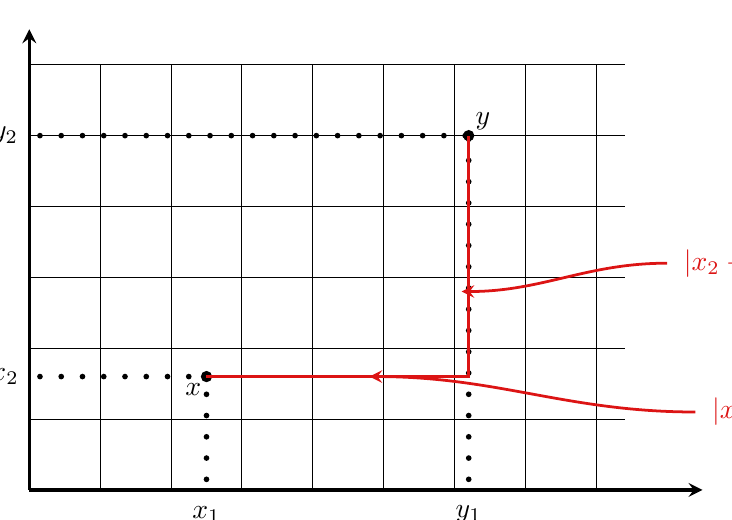
\begin{tikzpicture}[x=0.9cm,y=0.9cm,>=stealth]

    % 色
    \definecolor{myred}{RGB}{220,20,20}

    % パラメータ
    \def\xmax{9.5}
    \def\ymax{6.5}
    \def\xa{2.5}  % x_1
    \def\xb{1.6}  % x_2
    \def\ya{6.2}  % y_1
    \def\yb{5.0}  % y_2

    % グリッド
    \foreach \x in {0,1,...,8} {
        \draw[black,thin] (\x,0) -- (\x,6);
    }
    \foreach \y in {0,1,...,6} {
        \draw[black,thin] (0,\y) -- (8.4,\y);
    }

    % 座標軸
    \draw[black,line width=1.2pt,->] (0,0) -- (\xmax,0) node[right] {};
    \draw[black,line width=1.2pt,->] (0,0) -- (0,\ymax) node[above] {};

    % 点線の補助線をドットで表現
    \foreach \x in {0.15,0.45,...,\xa} {
        \fill (\x,\xb) circle (0.04);
    }
    \foreach \x in {0.15,0.45,...,\ya} {
        \fill (\x,\yb) circle (0.04);
    }
    \foreach \y in {0.15,0.45,...,\xb} {
        \fill (\xa,\y) circle (0.04);
    }
    \foreach \y in {0.15,0.45,...,\yb} {
        \fill (\ya,\y) circle (0.04);
    }

    % 点 x=(x_1,x_2), y=(y_1,y_2)
    \fill (\xa,\xb) circle (0.08);
    \fill (\ya,\yb) circle (0.08);

    % 赤い折れ線
    \draw[myred,line width=1.2pt] (\xa,\xb) -- (\ya,\xb) -- (\ya,\yb);

    % ラベル x, y
    \node[below left] at (\xa,\xb) {$x$};
    \node[above right] at (\ya,\yb) {$y$};

    % 軸上のラベル
    \node[left]  at (0,\xb) {$x_2$};
    \node[left]  at (0,\yb) {$y_2$};
    \node[below] at (\xa,0) {$x_1$};
    \node[below] at (\ya,0) {$y_1$};

    % 赤い注釈
    \draw[myred,line width=1.0pt,->]
        (9.0,3.2) to[out=180,in=0] (6.1,2.8);
    \node[myred,right] at (9.1,3.2) {$|x_2-y_2|$};

    \draw[myred,line width=1.0pt,->]
        (9.4,1.1) to[out=180,in=0] (4.8,1.6);
    \node[myred,right] at (9.5,1.1) {$|x_1-y_1|$};

\end{tikzpicture}
\vspace{1\baselineskip}
\caption{2次元の場合のマンハッタン距離の図}
\label{fig:n2-distance}
\end{figure}

\begin{figure}[htbp]
\centering

\begin{minipage}[t]{0.47\textwidth}
\centering

{\large 原点を通る同一直線上にあるとき}

\vspace{1em}

\begin{tikzpicture}[x=1cm,y=1cm,>=stealth]
    % 軸
    \draw[black,line width=1pt,->] (0.8,0.8) -- (5.8,0.8);
    \draw[black,line width=1pt,->] (0.8,0.8) -- (0.8,4.8);

    % 原点
    \fill (0.8,0.8) circle (0.07);
    \node[below left] at (0.8,0.8) {$0$};

    % 直線
    \draw[black,line width=1pt] (0.8,0.8) -- (4.7,3.8);

    % 点 x, y
    \fill (2.2,1.9) circle (0.07);
    \fill (3.9,3.2) circle (0.07);
    \node[below left] at (2.2,1.9) {$x$};
    \node[right] at (3.9,3.2) {$y$};

    % 距離
    \draw[red,line width=1pt] (2.2,1.9) -- (3.9,3.2);

    % 注釈
    \draw[red,line width=1pt,->]
        (5.6,2.0) to[out=180,in=-15] (3.0,2.55);
    \node[red,anchor=west] at (5.7,2.0) {$d_2^p(x,y)=d_2(x,y)$};

    \node[anchor=west] at (4.8,0.3) {通常のユークリッド距離};
\end{tikzpicture}
\end{minipage}
\hfill
\begin{minipage}[t]{0.47\textwidth}
\centering

{\large そうでないとき}

\vspace{1em}

\begin{tikzpicture}[x=1cm,y=1cm,>=stealth]
    % 軸
    \draw[black,line width=1pt,->] (0.8,0.8) -- (6.2,0.8);
    \draw[black,line width=1pt,->] (0.8,0.8) -- (0.8,4.8);

    % 原点
    \fill (0.8,0.8) circle (0.07);
    \node[below left] at (0.8,0.8) {$0$};

    % 半直線
    \draw[black,line width=1pt] (0.8,0.8) -- (2.4,3.4);
    \draw[black,line width=1pt] (0.8,0.8) -- (4.6,2.0);

    % 点 x, y
    \fill (1.8,2.5) circle (0.07);
    \fill (3.7,1.7) circle (0.07);
    \node[left] at (1.8,2.7) {$x$};
    \node[right] at (3.7,1.45) {$y$};

    % 原点経由の折れ線
    \draw[red,line width=1pt] (1.8,2.5) -- (0.8,0.8) -- (3.7,1.7);

    % 注釈
    \draw[red,line width=1pt,->]
        (4.8,3.4) to[out=180,in=15] (2.6,1.55);
    \node[black,anchor=west] at (4.9,3.4)
        {$d_2^p(x,y)=d_2(0,x)+d_2(0,y)$};

    \node[anchor=west] at (4.9,0.3) {原点を経由した距離};
\end{tikzpicture}
\end{minipage}

\vspace{1\baselineskip}
\caption{$\mathbb{R}^2$ におけるパリ距離の例}
\label{fig:d2p-minipage}
\end{figure}

\begin{ex}
    引き続き、さらに距離空間の例を挙げる :\\
    $f, g \in C([a,b])$ に対して、
    \begin{align*}
        d_{1}(f,g) &= \int_a^b \left\lvert f(x) - g(x) \right\rvert \,dx \\
        d_{2}(f,g) &= \sqrt{\int_a^b \left\lvert f(x) - g(x) \right\rvert^2 \,dx}
    \end{align*}
    と定めると、$d_{1}, d_{2}$ は $C([a,b])$ に距離を定める。
\end{ex}

\section{点列の収束と極限}

$\N$ を正の整数全体の集合とする。

\begin{dfn}
    $(X,d)$ を距離空間とする。
    \begin{itemize}
        \item 点列 $\{x_n\}_{n \in \N}$ が $x \in X$ に\textbf{収束}するとは、任意の $\varepsilon > 0$ に対して、ある $N \in \N$ が存在して、任意の $n \geq N$ に対して $d(x_n,x) < \varepsilon$ を満たすことをいう。つまり、
        \[\forall \varepsilon > 0, \exists N \in \N, \forall n \geq N, d(x_n,x) < \varepsilon\]
        を満たすことをいう。$x$ を点列 $\{x_n\}_{n \in \N}$ の\textbf{極限}と呼び、$\lim_{n \to \infty} x_n = x$ や $x_n \to x \, (n \to \infty)$ と表記する。
        \item $X$ 上の点列 $\{x_n\}_{n\in \N}$ と $\N$ の無限部分集合 $I$ に対して、点列 $\{x_n\}_{n \in I}$ を\textbf{部分列}と呼ぶ。
    \end{itemize}
\end{dfn}

\begin{prop}
以下が成り立つ :
\begin{enumerate}[label=(\arabic*)\,]
    \item 点列 $\{x_n\}_{n \in \N}$ が $x$ に収束するならば、$x$ は $\{x_n\}_{n \in \N}$ の唯一の極限である。つまり、点列の極限は一意である。
    \item 任意の $n \in \N$ に対して $x_n = x$ であるとき、点列 $\{x_n\}_{n \in \N}$ は $x$ に収束する。
    \item 点列 $\{x_n\}_{n \in \N}$ が $x$ に収束するならば、任意の部分列 $\{x_{i(n)}\}_{n \in I}$ も $x$ に収束する。
    \item 点列 $\{x_n\}_{n \in \N}$ の任意の部分列 $\{x_{i(n)}\}_{n \in I}$ が $x$ に収束するならば、点列 $\{x_n\}_{n \in \N}$ も $x$ に収束する。
    \item 点列 $\{x_n\}_{n \in \N}$ に対し、ある $\delta > 0$ が存在して、任意の $n \in \N$ に対して $d(x_n, x) \geq \delta$ が成り立つならば、点列 $\{x_n\}_{n \in \N}$ の任意の部分列 $\{x_{i(n)}\}_{n \in I}$ は収束しない。
\end{enumerate}
\end{prop}

\begin{proof}
(1) : 点列 $\{x_n\}_{n \in \N}$ が $x$ に収束するならば、任意の $\varepsilon > 0$ に対して、ある $N \in \N$ が存在して、任意の $n \geq N$ に対して $d(x_n,x) < \varepsilon$ を満たす。

もし、点列 $\{x_n\}_{n \in \N}$ が $y$ にも収束すると仮定すると、同様に、任意の $\varepsilon > 0$ に対して、ある $M \in \N$ が存在して、任意の $n \geq M$ に対して $d(x_n,y) < \varepsilon$ を満たす。ここで、$\varepsilon > 0$ を任意に取るとき、ある $K = \max\{N,M\} \in \N$ が存在して、任意の $n \geq K$ に対して、
\begin{align*}
d(x,y) &\leq d(x,x_n) + d(x_n,y) \\
&< \varepsilon + \varepsilon \\
&= 2\varepsilon
\end{align*}
を満たす。$\varepsilon$ は任意であるため、$d(x,y) = 0$ を満たす。距離空間の定義より、$y = x$ である。したがって、点列 $\{x_n\}_{n \in \N}$ の極限は一意である。

\vspace{1\baselineskip}

(2) : 任意の $n \in \N$ に対して $x_n = x$ であるとき、任意の $\varepsilon > 0$ に対して、任意の $n \in \N$ に対して $d(x_n,x) = d(x,x) = 0 < \varepsilon$ を満たす。したがって、点列 $\{x_n\}_{n \in \N}$ は $x$ に収束する。

\vspace{1\baselineskip}

(3) : 点列 $\{x_n\}_{n \in \N}$ が $x$ に収束するならば、任意の $\varepsilon > 0$ に対して、ある $N \in \N$ が存在して、任意の $n \geq N$ に対して $d(x_n,x) < \varepsilon$ を満たす。$\{x_{i(n)}\}_{n \in I}$ を $\{x_n\}_{n \in \N}$ の部分列とすると、$i(n) \geq n$ であるから、任意の $n \geq N$ に対して $d(x_{i(n)},x) < \varepsilon$ を満たす。したがって、部分列 $\{x_{i(n)}\}_{n \in I}$ も $x$ に収束する。

\vspace{1\baselineskip}

(4) : 背理法で示す。

もし点列 $\{x_n\}_{n \in \N}$ が $x$ に収束しないと仮定すると、ある $\varepsilon > 0$ が存在して、任意の $N \in \N$ が存在して、ある $n \geq N$ が存在して、$d(x_n,x) \geq \varepsilon$ を満たす。ここで、$\{n_k\}_{k\in\N}$ をこの条件を満たすように選んだ点列とすると、部分列 $\{x_{n_k}\}_{k\in\N}$ は $x$ に収束しない。これは背理法の仮定に反する。したがって、点列 $\{x_n\}_{n \in \N}$ も $x$ に収束する。

\vspace{1\baselineskip}

(5) : 背理法で示す。

もし点列 $\{x_n\}_{n \in \N}$ のある部分列 $\{x_{i(n)}\}_{n \in I}$ が $x$ に収束すると仮定する。
すると、任意の $\varepsilon > 0$ に対して、ある $N \in \N$ が存在して、任意の $n \geq N$ に対して $d(x_n,x) < \varepsilon$ を満たす。$\{x_{i(n)}\}_{n \in I}$ は $\{x_n\}_{n \in \N}$ の部分列なので $i(n) \geq n$ であるから、任意の $n \geq N$ に対して $d(x_{i(n)},x) < \varepsilon$ を満たす。しかし、$\varepsilon$ は任意であるため、ある $\delta > 0$ が存在して、任意の $n \in \N$ に対して $d(x_n,x) \geq \delta$ を満たすという仮定に矛盾する。したがって、点列 $\{x_n\}_{n \in \N}$ の任意の部分列 $\{x_{i(n)}\}_{n \in I}$ は収束しない。
\end{proof}

\lecture{第3回 : (2026/04/28)}

\section{平面 \texorpdfstring{$\R^2$}{R2} 上の点列}
\begin{thm}
    \quad $\{(x_n,y_n)\}$ : $\R^2$ 上の点列, $(\R^2,d)$ : 2次元ユークリッド空間.\\
   このとき、
   \[\lim_{n \to \infty} (x_n,y_n) = (x,y)\]
   であることと、
   \[\lim_{n \to \infty} x_n = x, \quad \lim_{n \to \infty} y_n = y\]
   であることは同値である。
\end{thm}

\begin{proof}
    $\Rightarrow$ : $\lim_{n \to \infty} (x_n,y_n) = (x,y)$ とする。任意の $\varepsilon > 0$ に対して、ある $N \in \N$ が存在して、任意の $n \geq N$ に対して、
    \begin{align*}
        d((x_n,y_n),(x,y)) &= \sqrt{(x_n - x)^2 + (y_n - y)^2} < \varepsilon
    \end{align*}
    を満たす。ここで、$\sqrt{(x_n - x)^2 + (y_n - y)^2} < \varepsilon$ であるから、$\left\lvert x_n - x \right\rvert < \varepsilon$ および $\left\lvert y_n - y \right\rvert < \varepsilon$ を満たす。したがって、$\lim_{n \to \infty} x_n = x$ および $\lim_{n \to \infty} y_n = y$ である。

    $\Leftarrow$ : $\lim_{n \to \infty} x_n = x, \quad \lim_{n \to \infty} y_n = y$ とする。任意の $\varepsilon > 0$ に対して、ある $N_1, N_2 \in \N$ が存在して、任意の $n \geq N_1$ に対して $\left\lvert x_n - x\right\rvert < \varepsilon/\sqrt{2}$ を満たし、任意の $n \geq N_2$ に対して $\left\lvert y_n - y\right\rvert < \varepsilon/\sqrt{2}$ を満たす。ここで、ある $N = \max\{N_1,N_2\} \in \N$ が存在して、任意の $n \geq N$ に対して、
    \begin{align*}
        d((x_n,y_n),(x,y)) &= \sqrt{(x_n - x)^2 + (y_n - y)^2} < \sqrt{\left(\frac{\varepsilon}{\sqrt{2}}\right)^2 + \left(\frac{\varepsilon}{\sqrt{2}}\right)^2} = \varepsilon
    \end{align*}
    を満たす。したがって、$\lim_{n \to \infty} (x_n,y_n) = (x,y)$ である。
\end{proof}

\begin{lem}\label{lem:distance-comparison}
    \quad $X$ : 集合, $d, d^{\prime}$ : $X$ 上の距離.\\
    ここで、ある $k > 0$ が存在して、任意の $x,y \in X$ に対して、
    \[d(x,y) \leq k\cdot d^{\prime}(x,y)\]
    を満たすとする。このとき、点列 $\{x_n\}_{n \in \N}$ が $x$ に対して $d$ によって収束するならば、点列 $\{x_n\}_{n \in \N}$ は $x$ に対して $d^{\prime}$ によっても収束する。
\end{lem}

\begin{proof}
    点列 $\{x_n\}_{n \in \N}$ が $x$ に対して $d$ によって収束するならば、任意の $\varepsilon > 0$ に対して、ある $N \in \N$ が存在して、任意の $n \geq N$ に対して $d(x_n,x) < \varepsilon$ を満たす。ここで、ある $k > 0$ が存在して、任意の $x,y \in X$ に対して $d(x,y) \leq k\cdot d^{\prime}(x,y)$ を満たすので、任意の $n \geq N$ に対して、
    \[d^{\prime}(x_n,x) \leq k\cdot d(x_n,x) < k\cdot \varepsilon\]
    を満たす。$\varepsilon$ は任意であるため、点列 $\{x_n\}_{n \in \N}$ は $x$ に対して $d^{\prime}$ によっても収束する。
\end{proof}

\begin{figure}[htbp]
\centering
\begin{tikzpicture}[
  scale=1.0,
  line cap=round,
  line join=round,
  >=Stealth,
  every node/.style={font=\large}
]

% center point
\coordinate (x0) at (4.3,2.0);

% ambient space X
\draw[line width=1.4pt]
  (0.2,1.75)
  .. controls (0.35,2.45) and (0.75,2.95) .. (1.25,2.95)
  .. controls (2.30,2.90) and (2.60,2.75) .. (3.75,3.10)
  .. controls (5.15,3.55) and (6.25,3.55) .. (7.25,2.95)
  .. controls (8.00,2.45) and (8.25,1.55) .. (7.70,0.95)
  .. controls (7.25,0.45) and (6.15,0.25) .. (5.25,0.05)
  .. controls (4.40,-0.10) and (3.85,0.20) .. (3.55,0.35)
  .. controls (2.75,0.45) and (2.55,0.20) .. (2.15,0.40)
  .. controls (1.25,0.15) and (0.45,0.45) .. (0.15,1.15)
  .. controls (0.05,1.35) and (0.10,1.55) .. cycle;

% label X
\node at (0.35,3.55) {$X$};

% outer green neighborhood
\draw[black, line width=1.4pt]
  (x0) ellipse [x radius=1.55, y radius=0.85];

% inner orange neighborhood
\draw[black, line width=1.4pt]
  (x0) ellipse [x radius=0.62, y radius=0.52];

% point x_0
\fill (x0) circle (3.5pt);
\node[right=2pt] at (x0) {\large $x_0$};

% green arrow and label
\draw[black, line width=1.4pt, ->]
  (6.95,2.65) .. controls (6.55,2.55) and (6.25,2.35) .. (5.85,2.25);

\node[black, right] at (7.15,2.55)
  {\large $U_d\!\left(x_0;\dfrac{\varepsilon}{k}\right)$};

% orange arrow and label
\draw[black, line width=1.4pt, ->]
  (3.78,0.95) .. controls (3.65,1.30) and (3.72,1.63) .. (3.95,1.75);

\node[black, below] at (5,1)
  {\large $U_{d'}(x_0;\varepsilon)$};

\end{tikzpicture}
\end{figure}

\begin{prop}
    \quad $\{p_n\}$ : $\R^2$ 上の点列, $X \in \R^2$ : 点.\\
    \quad $d_2$ : 2次元ユークリッド距離, $d_2^P$ : 2次元パリ距離, $d_{2}^{F}$ : 2次元チェビシェフ距離.\\
    このとき、次は同値である : 
\begin{enumerate}[label=(\arabic*)\,]
    \item 点列 $\{p_n\}$ は $X$ に対して $d_2$ によって収束する。
    \item 点列 $\{p_n\}$ は $X$ に対して $d_{2}^{P}$ によって収束する。
    \item 点列 $\{p_n\}$ は $X$ に対して $d_{2}^{F}$ によって収束する。
    \end{enumerate}
\end{prop}

\begin{proof}
    (1) $\Rightarrow$ (2) : 任意の $(x,y), (x^{\prime},y^{\prime}) \in \R^2$ に対して、
    \begin{align*}
        d_2^P((x,y),(x^{\prime},y^{\prime})) &\leq d_2((x,y),(x^{\prime},y^{\prime})) \\
        &\leq \sqrt{2}\cdot d_2^P((x,y),(x^{\prime},y^{\prime}))
    \end{align*}
    を満たす。したがって、補題\ref{lem:distance-comparison}より、点列 $\{p_n\}$ は $X$ に対して $d_2^P$ によって収束する。\\
    
    (2) $\Rightarrow$ (3) : 任意の $(x,y), (x^{\prime},y^{\prime}) \in \R^2$ に対して、
    \begin{align*}
        d_{2}^{F}((x,y),(x^{\prime},y^{\prime})) &\leq d_2^P((x,y),(x^{\prime},y^{\prime})) \\
        &\leq 2\cdot d_{2}^{F}((x,y),(x^{\prime},y^{\prime}))
    \end{align*}
    を満たす。したがって、補題\ref{lem:distance-comparison}より、点列 $\{p_n\}$ は $X$ に対して $d_{2}^{F}$ によって収束する。\\
    
    (3) $\Rightarrow$ (1) : 任意の $(x,y), (x^{\prime},y^{\prime}) \in \R^2$ に対して、
    \begin{align*}
        d_2((x,y),(x^{\prime},y^{\prime})) &\leq \sqrt{2}\cdot d_{2}^{F}((x,y),(x^{\prime},y^{\prime})) \\
        &\leq 2\cdot d_2((x,y),(x^{\prime},y^{\prime}))
    \end{align*}
    を満たす。したがって、補題\ref{lem:distance-comparison}より、点列 $\{p_n\}$ は $X$ に対して $d_2$ によって収束する。
\end{proof}

\begin{ex}
    上の状況で、各 $n$ に対し、$p_n = \left(1, \frac{1}{n}\right)$ , $X = (1,0)$ とする。すると、点列 $\{p_n\}$ は $X$ に対して $d_2$ によって収束するが、点列 $\{p_n\}$ は $X$ に対して $d_{2}^{P}$ によって収束しない。\\

    実際、任意の $n \in \N$ に対して、
    \begin{align*}
        d_2(p_n,X) &= \sqrt{\left(1 - 1\right)^2 + \left(\frac{1}{n} - 0\right)^2} = \frac{1}{n} \to 0 \quad (n \to \infty) \\
        d_2^P(p_n,X) &=
        d_2(p_n, (0,0)) + d_2((0,0),X) \\
        &= \sqrt{1^2 + \left(\frac{1}{n}\right)^2} + \sqrt{1^2 + 0^2} \\
        &= \sqrt{1 + \frac{1}{n^2}} + 1 \to 2 \quad (n \to \infty)
    \end{align*}   
    を満たす。 したがって、点列 $\{p_n\}$ は $X$ に対して $d_2$ によって収束するが、点列 $\{p_n\}$ は $X$ に対して $d_{2}^{P}$ によって収束しない。
\end{ex}

\begin{ex}
    $X$ : 集合, $p_{0}(x,y) := \begin{cases}
        0 \quad & (x=y) \\
        1 \quad & (x \neq y)
    \end{cases}$.\\
    $p_{0}$ は $X$ 上の距離を定める。この距離空間 $(X, p_0)$ を\textbf{離散距離空間}と呼ぶ。\\
    \quad 任意の点列 $\{x_n\}_{n \in \N}$ と点 $x \in X$ に対して、点列 $\{x_n\}_{n \in \N}$ は $x$ に対して $p_0$ によって収束するならば、ある $N \in \N$ が存在して、任意の $n \geq N$ に対して $x_n = x$ を満たす。逆に、ある $N \in \N$ が存在して、任意の $n \geq N$ に対して $x_n = x$ を満たすならば、点列 $\{x_n\}_{n \in \N}$ は $x$ に対して $p_0$ によって収束する。したがって、点列 $\{x_n\}_{n \in \N}$ は $x$ に対して $p_0$ によって収束することと、ある $N \in \N$ が存在して、任意の $n \geq N$ に対して $x_n = x$ を満たすことは同値である。
\end{ex}

\section{距離空間の開集合}

\begin{dfn}
    \quad $(X,d)$ : 距離空間, $x \in X$ : 点, $\varepsilon > 0$.\\
    \[U_d(x;\varepsilon) := \{y \in X \mid d(x,y) \leq  \varepsilon\}\]
    を $X$ 上の点 $x$ と実数 $\varepsilon$ に対する$\varepsilon$\textbf{-\hspace{0pt}近傍}と呼ぶ。、$U(x;\varepsilon)$ と略記することもある。
\end{dfn}

\begin{ex}
    \quad $(\R^2, d_2)$ : 2次元ユークリッド距離空間, $x = (0,0)$ : 点, $\varepsilon > 0$.\\
    このとき、$U_{d_2}(x;\varepsilon)$ は原点を中心とする半径 $\varepsilon$ の円盤の内部である。
\end{ex}

\begin{figure}[htbp]
\centering
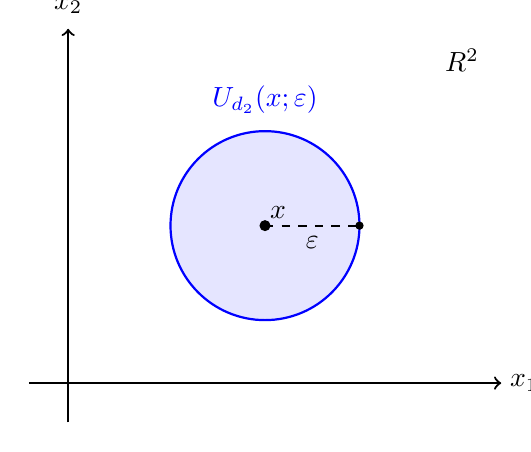
\begin{tikzpicture}[scale=1.0]

  % 座標軸
  \draw[->,thick] (-0.5,0) -- (5.5,0) node[right] {$x_1$};
  \draw[->,thick] (0,-0.5) -- (0,4.5) node[above] {$x_2$};

  % 点 x の位置
  \coordinate (x) at (2.5,2);

  % 近傍 U_{d_2}(x;\varepsilon)
  \filldraw[fill=blue!10, draw=blue, thick] (x) circle (1.2);

  % 中心点 x
  \fill (x) circle (2pt);
  \node[above right] at (x) {$x$};

  % 半径 epsilon を示す点
  \coordinate (p) at (3.7,2);

  % 半径の線
  \draw[dashed,thick] (x) -- (p);
  \node[below] at ($(x)!0.5!(p)$) {$\varepsilon$};

  % 円周上の点（任意）
  \fill (p) circle (1.5pt);

  % 集合名
  \node[blue] at (2.5,3.6) {$U_{d_2}(x;\varepsilon)$};

  % 空間のラベル
  \node at (5.0,4.1) {$\mathbb{R}^2$};
\end{tikzpicture}
\end{figure}

\begin{ex}
    \quad $(\R^3, d_3)$ : 3次元ユークリッド距離空間, $x = (0,0,0)$ : 点, $\varepsilon > 0$.\\
    このとき、$U_{d_3}(x;\varepsilon)$ は原点を中心とする半径 $\varepsilon$ の球体の内部である。
\end{ex}

\vspace{1\baselineskip}

\begin{figure}[htbp]
  \centering
  \begin{tikzpicture}[scale=1.2, >=Stealth, line cap=round, line join=round]

    \coordinate (O) at (0,0);
    \def\R{2.2}

    \shade[ball color=blue!15, opacity=0.8] (O) circle (\R);
    \draw[thick] (O) circle (\R);

    \draw[dashed] (-\R,0) arc[start angle=180,end angle=360,x radius=\R,y radius=0.65];
    \draw[thick]   (\R,0) arc[start angle=0,end angle=180,x radius=\R,y radius=0.65];

    \fill (O) circle (2pt);
    \node at (0,-1) {$x=(0,0,0)$};

    \coordinate (P) at ({\R*cos(35)},{\R*sin(35)});
    \draw[thick,->] (O) -- (P);
    \node[midway, above right] {$\varepsilon$};

    \node at (3,2) {$U_{d_3}(x;\varepsilon)$};

  \end{tikzpicture}
  \caption{$U_{d_3}(x;\varepsilon)$ は原点を中心とする半径 $\varepsilon$ の開球である。}
\end{figure}

\begin{ex}
    \quad $(\R^2, d_2^P)$ : 2次元パリ距離空間, $x = (0,0)$ : 点, $\varepsilon > 0$.\\
    このとき、$U_{d_2^P}(x;\varepsilon)$ は原点を中心とする半径 $\varepsilon$ の正方形の内部である。つまり、
    \[U_{d_2^P}(x;\varepsilon) = \{(x,y) \in \R^2 \mid |x| + |y| < \varepsilon\}\]
    である。
\end{ex}

\begin{figure}[htbp]
  \centering
  \begin{tikzpicture}[scale=1.2, >=Stealth]

    \def\eps{2}


    % 開球
    \filldraw[fill=blue!10, draw=blue, thick]
      (0,\eps) -- (\eps,0) -- (0,-\eps) -- (-\eps,0) -- cycle;

    % 原点
    \fill (0,0) circle (2pt);
    \node[below left,font=\small] at (-0.1,-0.05) {$x=(0,0)$};

    % 頂点ラベル
    \node[above right] at (0.1,\eps) {$(0,\varepsilon)$};
    \node[above right] at (\eps,0.1) {$(\varepsilon,0)$};
    \node[below right] at (0.1,-\eps) {$(0,-\varepsilon)$};
    \node[above left] at (-\eps,0.1) {$(-\varepsilon,0)$};

    % 集合名
    \node[blue] at (-3,2.55) {$U_{d_2^P}(x;\varepsilon)$};

    % 座標軸（実線）
    \draw[->, thick] (-2.8,0) -- (2.8,0) node[below right] {$x$};
    \draw[->, thick] (0,-2.8) -- (0,2.8) node[above left] {$y$};


  \end{tikzpicture}
  \caption{$U_{d_2^P}(x;\varepsilon)=\{(x,y)\in\mathbb{R}^2 \mid |x|+|y|<\varepsilon\}$}
\end{figure}

\begin{lem}
    \quad $(X,d)$ : 距離空間, $x \in X$ : 点\\
    このとき、次が成り立つ :
    \begin{enumerate}[label=(\arabic*)\,]
        \item 任意の $\varepsilon > 0$ に対して、$x \in U_d(x;\varepsilon)$ を満たす。
        \item 任意の $\varepsilon \geq \delta > 0$ に対して、$U_d(x;\delta) \subseteq U_d(x;\varepsilon)$ を満たす。
        \item 任意の $\varepsilon > 0$ に対して $y \in U_d(x;\varepsilon)$ ならば、ある $\delta > 0$ が存在して、$U_d(y;\delta) \subseteq U_d(x;\varepsilon)$ を満たす。
    \end{enumerate}
\end{lem}

\begin{proof}[(1)の証明]
    任意の $\varepsilon > 0$ に対して、$d(x,x) = 0 < \varepsilon$ を満たす。したがって、$x \in U_d(x;\varepsilon)$ を満たす。
\end{proof}

\begin{proof}[(2)の証明]
    任意の $\varepsilon \geq \delta > 0$ に対して、任意の $y \in U_d(x;\delta)$ に対して $d(x,y) < \delta \leq \varepsilon$ を満たす。したがって、$U_d(x;\delta) \subseteq U_d(x;\varepsilon)$ を満たす。
\end{proof}

\begin{proof}[(3)の証明]
    任意の $\varepsilon > 0$ に対して $y \in U_d(x;\varepsilon)$ ならば、$d(x,y) < \varepsilon$ を満たす。したがって、$\delta = \varepsilon - d(x,y) > 0$ とおくと、任意の $z \in U_d(y;\delta)$ に対して $d(y,z) < \delta$ を満たす。よって、
    \[d(x,z) \leq d(x,y) + d(y,z) < d(x,y) + (\varepsilon - d(x,y)) = \varepsilon\]
    を満たす。したがって、$U_d(y;\delta) \subseteq U_d(x;\varepsilon)$ を満たす。
\end{proof}

\begin{dfn}
    \quad $(X,d)$ : 距離空間, $U \subseteq X$.\\
    $U$ が $X$ の\textbf{開集合}であるとは、任意の $x \in U$ に対して、ある $\varepsilon > 0$ が存在して $U_d(x;\varepsilon) \subseteq U$ を満たすことをいう。
\end{dfn}

\begin{prop}
    \quad $(X,d)$ : 距離空間.\\
    このとき、任意の $\varepsilon > 0$ に対して、$U_d(x;\varepsilon)$ は $X$ の開集合である。
\end{prop}

\begin{proof}
    任意の $y \in U_d(x;\varepsilon)$ に対して、$d(x,y) < \varepsilon$ を満たす。したがって、$\delta = \varepsilon - d(x,y) > 0$ とおくと、任意の $z \in U_d(y;\delta)$ に対して $d(y,z) < \delta$ を満たす。よって、
    \[d(x,z) \leq d(x,y) + d(y,z) < d(x,y) + (\varepsilon - d(x,y)) = \varepsilon\]
    を満たす。したがって、$U_d(y;\delta) \subseteq U_d(x;\varepsilon)$ を満たす。したがって、任意の $y \in U_d(x;\varepsilon)$ に対して、ある $\delta > 0$ が存在して $U_d(y;\delta) \subseteq U_d(x;\varepsilon)$ を満たす。したがって、$U_d(x;\varepsilon)$ は $X$ の開集合である。
\end{proof}

\begin{thm}
    \quad $(X,d)$ : 距離空間, $U \subseteq X$.\quad このとき、次の性質が成り立つ : 
    \begin{enumerate}[label=(\arabic*)\,]
        \item $X$ と $\emptyset$ は $X$ の開集合である。
        \item 有限個の開集合 $\mathcal{O}_1, \mathcal{O}_2, \ldots, \mathcal{O}_n$ の和集合 $\bigcap_{i=1}^n \mathcal{O}_i$ は $X$ の開集合である。
        \item 任意の個数の開集合 $\{\mathcal{O}_i\}_{i \in I}$ の和集合 $\bigcup_{i \in I} \mathcal{O}_i$ は $X$ の開集合である。
    \end{enumerate}
\end{thm}

\begin{proof}[(1)の証明]
    任意の $x \in X$ に対して、ある $\varepsilon > 0$ が存在して $U_d(x;\varepsilon) \subseteq X$ を満たす。したがって、$X$ は $X$ の開集合である。

    $\emptyset$ は空集合であるから、任意の $x \in \emptyset$ に対して、ある $\varepsilon > 0$ が存在して $U_d(x;\varepsilon) \subseteq \emptyset$ を満たす。したがって、$\emptyset$ は $X$ の開集合である。
\end{proof}

\begin{proof}[(2)の証明]
    任意の $x \in \bigcap_{i=1}^n \mathcal{O}_i$ に対して、任意の $1 \leq i \leq n$ に対して $x \in \mathcal{O}_i$ を満たす。したがって、任意の $1 \leq i \leq n$ に対して、ある $\varepsilon_i > 0$ が存在して $U_d(x;\varepsilon_i) \subseteq \mathcal{O}_i$ を満たす。ここで、$\varepsilon = \min\{\varepsilon_1, \varepsilon_2, \ldots, \varepsilon_n\} > 0$ とおくと、任意の $1 \leq i \leq n$ に対して $U_d(x;\varepsilon) \subseteq U_d(x;\varepsilon_i) \subseteq \mathcal{O}_i$ を満たす。したがって、任意の $1 \leq i \leq n$ に対して $U_d(x;\varepsilon) \subseteq \mathcal{O}_i$ を満たす。したがって、$U_d(x;\varepsilon) \subseteq \bigcap_{i=1}^n \mathcal{O}_i$ を満たす。したがって、$\bigcap_{i=1}^n \mathcal{O}_i$ は $X$ の開集合である。
\end{proof}

\begin{proof}[(3)の証明]
    任意の $x \in \bigcup_{i \in I} \mathcal{O}_i$ に対して、ある $i_0 \in I$ が存在して $x \in \mathcal{O}_{i_0}$ を満たす。したがって、ある $\varepsilon > 0$ が存在して $U_d(x;\varepsilon) \subseteq \mathcal{O}_{i_0}$ を満たす。したがって、$U_d(x;\varepsilon) \subseteq \bigcup_{i \in I} \mathcal{O}_i$ を満たす。したがって、$\bigcup_{i \in I} \mathcal{O}_i$ は $X$ の開集合である。
\end{proof}

\lecture{第4回 : (2026/05/12)}

\begin{ex}
    \quad $(\R^2, d_2)$ : 2次元ユークリッド距離空間, $x = (0,0) \in \R^2$, $\mathcal{O}_i = U\left(x,\frac{1}{i}\right)$.\\
    このとき、$\bigcap_{i=1}^{\infty} \mathcal{O}_i = \{x\}$ である。したがって、$\bigcap_{i=1}^{\infty} \mathcal{O}_i$ は $X$ の開集合ではない。
    \begin{proof}[$\subseteq$に関して : ]
        任意の $y \in \bigcap_{i=1}^{\infty} \mathcal{O}_i$ に対して、任意の $i \in \N$ に対して $y \in U\left(x,\frac{1}{i}\right)$ を満たす。したがって、任意の $i \in \N$ に対して $d(x,y) < \frac{1}{i}$ を満たす。$\frac{1}{i} \to 0$ (as $i \to \infty$) であるから、$d(x,y) = 0$ を満たす。したがって、$y = x$ を満たす。したがって、$\bigcap_{i=1}^{\infty} \mathcal{O}_i \subseteq \{x\}$ を満たす。
    \end{proof}
    \begin{proof}[$\supseteq$に関して : ]
        任意の $i \in \N$ に対して、$d(x,x) = 0 < \frac{1}{i}$ を満たすので任意の $i \in \N$ に対して $x \in U\left(x,\frac{1}{i}\right)$ を満たす。よって、$x \in \bigcap_{i=1}^{\infty} \mathcal{O}_i$ を満たし、したがって、$\{x\} \subseteq \bigcap_{i=1}^{\infty} \mathcal{O}_i$ を満たす。
    \end{proof}
\end{ex}

\begin{prop}
    \quad $(\R^2, d_2)$ : 2次元ユークリッド距離空間, $A \subseteq \R^2$.\\
    このとき、以下は同値である : 
    \begin{enumerate}[label=(\arabic*)\,]
        \item $A$ は $(\R^2, d_2)$ の開集合である。
        \item $A$ は $(\R^2, d_2^P)$ の開集合である。
        \item $A$ は $(\R^2, d_{2}^{F})$ の開集合である。
        \item 
    \end{enumerate}
\end{prop}

\begin{proof}[(1) $\Rightarrow$ (2)の証明]
    $A$ は $(\R^2, d_2)$ の開集合であるから、任意の $x \in A$ に対して、ある $\varepsilon > 0$ が存在して $U_{d_2}(x;\sqrt{2}\varepsilon) \subseteq A$ を満たす。ここで、補題\ref{lem:distance-comparison}より、任意の $y \in U_{d_2^P}(x;\varepsilon)$ に対して 
    \[d_2(x,y) \leq \sqrt{2}\cdot d_{d_2^P}(x,y) < \sqrt{2}\varepsilon\]
    を満たす。もし、$d_{d_2^P}(x,y) < \varepsilon$ を満たすならば、$d_2(x,y) < \sqrt{2}\varepsilon$ を満たすので、
    \[U_{d_2^P}(x;\varepsilon) \subseteq U_{d_2}(x;\sqrt{2}\varepsilon) \subseteq A\]
    を満たす。したがって、任意の $x \in A$ に対して、ある $\varepsilon > 0$ が存在して $U_{d_2^P}(x;\varepsilon) \subseteq A$ を満たす。したがって、$A$ は $(\R^2, d_2^P)$ の開集合である。
\end{proof}

\begin{proof}[(2) $\Rightarrow$ (1)の証明]
    $A$ は $(\R^2, d_2^P)$ の開集合であるから、任意の $x \in A$ に対して、ある $\varepsilon > 0$ が存在して $U_{d_2^P}(x;\sqrt{2}\varepsilon) \subseteq A$ を満たす。ここで、補題\ref{lem:distance-comparison}より、任意の $y \in U_{d_2}(x;\varepsilon)$ に対して
    \[d_{d_2^P}(x,y) \leq d_2(x,y) < \varepsilon\]
    を満たす。もし、$d_2(x,y) < \varepsilon$ を満たすならば、$d_{d_2^P}(x,y) < \varepsilon$ を満たすので、
    \[U_{d_2}(x;\varepsilon) \subseteq U_{d_2^P}(x;\sqrt{2}\varepsilon) \subseteq A\]
    を満たす。したがって、任意の $x \in A$ に対して、ある $\varepsilon > 0$ が存在して $U_{d_2}(x;\varepsilon) \subseteq A$ を満たす。したがって、$A$ は $(\R^2, d_2)$ の開集合である。
\end{proof}

\begin{proof}[(1) $\Rightarrow$ (3)の証明]
    $A$ は $(\R^2, d_2)$ の開集合であるから、任意の $x \in A$ に対して、ある $\varepsilon > 0$ が存在して $U_{d_2}(x;\sqrt{2}\varepsilon) \subseteq A$ を満たす。ここで、補題\ref{lem:distance-comparison}より、任意の $y \in U_{d_2^F}(x;\varepsilon)$ に対して
    \[d_2(x,y) \leq \sqrt{2}\cdot d_{d_2^F}(x,y) < \sqrt{2}\varepsilon\]
    を満たす。もし、$d_{d_2^F}(x,y) < \varepsilon$ を満たすならば、$d_2(x,y) < \sqrt{2}\varepsilon$ を満たすので、
    \[U_{d_2^F}(x;\varepsilon) \subseteq U_{d_2}(x;\sqrt{2}\varepsilon) \subseteq A\]
    を満たす。したがって、任意の $x \in A$ に対して、ある $\varepsilon > 0$ が存在して $U_{d_2^F}(x;\varepsilon) \subseteq A$ を満たす。したがって、$A$ は $(\R^2, d_{2}^{F})$ の開集合である。
\end{proof}

\begin{proof}[(3) $\Rightarrow$ (1)の証明]
    $A$ は $(\R^2, d_{2}^{F})$ の開集合であるから、任意の $x \in A$ に対して、ある $\varepsilon > 0$ が存在して $U_{d_2^F}(x;\varepsilon) \subseteq A$ を満たす。ここで、補題\ref{lem:distance-comparison}より、任意の $y \in U_{d_2}(x;\varepsilon)$ に対して
    \[d_{d_2^F}(x,y) \leq d_2(x,y) < \varepsilon\]
    を満たす。もし、$d_2(x,y) < \varepsilon$ を満たすならば、$d_{d_2^F}(x,y) < \varepsilon$ を満たすので、
    \[U_{d_2}(x;\varepsilon) \subseteq U_{d_2^F}(x;\varepsilon) \subseteq A\]
    を満たす。したがって、任意の $x \in A$ に対して、ある $\varepsilon > 0$ が存在して $U_{d_2}(x;\varepsilon) \subseteq A$ を満たす。したがって、$A$ は $(\R^2, d_2)$ の開集合である。
\end{proof}

\section{位相空間}

\begin{dfn}
    \quad $X$ : 集合, $\mathcal{J}$ : $X$ の部分集合の族.\\
    $(X, \mathcal{J})$ は\textbf{位相空間}であるとは、$\mathcal{J}$ が、次の性質を満たすことをいう :
\begin{enumerate}[label=(\arabic*)\,]
    \item $X, \emptyset \in \mathcal{J}$
    \item 有限個の集合 $\mathcal{O}_1, \mathcal{O}_2, \ldots, \mathcal{O}_n \in \mathcal{J}$ に対して、$\bigcap_{i=1}^n \mathcal{O}_i \in \mathcal{J}$
    \item 任意の集合 $\mathcal{O}_\alpha \in \mathcal{J}$ に対して、$\bigcup_{\alpha} \mathcal{O}_\alpha \in \mathcal{J}$
\end{enumerate}
このとき、$\mathcal{J}$ の元を $X$ の\textbf{開集合}と呼び、$\mathcal{J}$ を $X$ の\textbf{位相}と呼ぶ。
\end{dfn}

\begin{ex}
    \quad $(X,d)$ : 距離空間.\\
    このとき、$X$ の開集合全体の集合 $\mathcal{J}_d$ は $X$ の位相を定める。つまり、$(X, \mathcal{J}_d)$ は位相空間である。
\end{ex}

\section{部分空間と直積空間}

\begin{dfn}
    \quad $(X,d)$ : 距離空間, $Y \subseteq X$ : 部分集合.\\
    $Y$ 上の距離 $d_Y$ を、任意の $y_1, y_2 \in Y$ に対して 
    \[d_Y(y_1,y_2) := d(y_1,y_2)\]
    と定めると、$(Y, d_Y)$ は距離空間である。$(Y, d_Y)$ を $(X,d)$ の\textbf{部分空間}と呼ぶ。
\end{dfn}

\begin{ex}
    \quad $(\R^m, d_m)$ : $m$ 次元ユークリッド距離空間, $n \in \Z_{>0}$, $0 < n < m$.\\
    このとき、$Y = \{(x_1, x_2, \ldots, x_m) \in \R^m \mid x_{n+1} = x_{n+2} = \cdots = x_m = 0\}$ と定めると、$(Y, d_Y)$ は $n$ 次元ユークリッド距離空間 $(\R^n, d_n)$ と同一視可能である。したがって、$(Y, d_Y)$ は $n$ 次元ユークリッド距離空間である。\\
    実際、任意の $y_1 = (x_1, x_2, \ldots, x_n, 0, 0, \ldots, 0), y_2 = (x_1^{\prime}, x_2^{\prime}, \ldots, x_n^{\prime}, 0, 0, \ldots, 0) \in Y$ に対して、
    \begin{align*}
        d_Y(y_1,y_2) &= \sqrt{(x_1 - x_1^{\prime})^2 + (x_2 - x_2^{\prime})^2 + \cdots + (x_n - x_n^{\prime})^2 + 0^2 + \cdots + 0^2} \\
        &= \sqrt{(x_1 - x_1^{\prime})^2 + (x_2 - x_2^{\prime})^2 + \cdots + (x_n - x_n^{\prime})^2} \\
        &= d_n((x_1, x_2, \ldots, x_n), (x_1^{\prime}, x_2^{\prime}, \ldots, x_n^{\prime}))
    \end{align*}
    を満たす。したがって、$(Y, d_Y)$ は $n$ 次元ユークリッド距離空間 $(\R^n, d_n)$ と同一視可能である。したがって、$(Y, d_Y)$ は $n$ 次元ユークリッド距離空間である。
\end{ex}

\begin{lem}
    \quad $(X,d)$ : 距離空間, $Y \subseteq X$ : 部分集合.\\
    このとき、任意の $y \in Y$ と $\varepsilon > 0$ に対して、
    \[U_{d_Y}(y;\varepsilon) = U_d(y;\varepsilon) \cap Y\]
    を満たす。
\end{lem}

\begin{proof}[$\subseteq$の証明]
    任意の $z \in U_{d_Y}(y;\varepsilon)$ に対して、$d_Y(y,z) < \varepsilon$ を満たす。したがって、$d(y,z) < \varepsilon$ を満たすので、$z \in U_d(y;\varepsilon)$ を満たす。また、$z \in Y$ を満たす。したがって、$z \in U_d(y;\varepsilon) \cap Y$ を満たす。したがって、$U_{d_Y}(y;\varepsilon) \subseteq U_d(y;\varepsilon) \cap Y$ を満たす。
\end{proof}

    
  \begin{proof}[$\supseteq$の証明]  
    任意の $z \in U_d(y;\varepsilon) \cap Y$ に対して、$d(y,z) < \varepsilon$ を満たす。したがって、$d_Y(y,z) < \varepsilon$ を満たすので、$z \in U_{d_Y}(y;\varepsilon)$ を満たす。したがって、$U_d(y;\varepsilon) \cap Y \subseteq U_{d_Y}(y;\varepsilon)$ を満たす。
\end{proof}

\begin{thm}
    \quad $(X,d)$ : 距離空間, $Y \subseteq X$ : 部分集合.\\
    このとき、$\mathcal{O} \subseteq Y$ が開集合であるための必要十分条件は、ある $\mathcal{O}^\prime \subseteq X$ が $(X,d)$ の開集合で、$\mathcal{O} = \mathcal{O}^\prime \cap Y$ を満たすことである。
\end{thm}

\begin{proof}[$\Longrightarrow$]
    任意の $\mathcal{O} \subseteq Y$ が開集合であるとする。このとき、$\mathcal{O} = \mathcal{O}^\prime \cap Y$ を満たす $(X,d)$ の開集合 $\mathcal{O}^\prime$ が存在する。
\end{proof}

\begin{proof}[$\Longleftarrow$]
    任意の $\mathcal{O} \subseteq Y$ が $\mathcal{O} = \mathcal{O}^\prime \cap Y$ を満たす $(X,d)$ の開集合 $\mathcal{O}^\prime$ が存在するとする。このとき、$\mathcal{O}$ は $Y$ の開集合である。
\end{proof}

\begin{dfn}
    \quad $(X,d_X), (Y,d_Y)$ : 距離空間.\\
    $X \times Y$ 上の距離 $d_{X \times Y}$ を、任意の $(x_1,y_1), (x_2,y_2) \in X \times Y$ に対して
    \[d_{X \times Y}((x_1,y_1),(x_2,y_2)) := \sqrt{d_X(x_1,x_2)^2 + d_Y(y_1,y_2)^2}\]
    と定めると、$(X \times Y, d_{X \times Y})$ は距離空間である。$(X \times Y, d_{X \times Y})$ を $X$ と $Y$ の\textbf{直積空間}と呼ぶ。
\end{dfn}
\end{document}
